% Nominal single-target comparison on N(2.2,2.2,pi/2).
% Values are taken directly from the run summaries and match Table III of the paper:
%   Adam (best horizon, 70 ns) : C=0.1576  F=0.99662  L=2.82e-4  T=70
%   TRPO nominal               : C=0.2982  F=0.99415  L=1.60e-3  T=116
%   TRPO noise-optimized       : C=0.1840  F=0.99876  L=2.12e-3  T=90
\documentclass[border=2pt]{standalone}
\usepackage[T1]{fontenc}
\usepackage{lmodern}
\usepackage{amsmath,amssymb}
\usepackage{pgfplots}
\pgfplotsset{compat=1.18}
\usepgfplotslibrary{groupplots}

\definecolor{cAdam}{RGB}{31,78,160}
\definecolor{cNom}{RGB}{224,109,30}
\definecolor{cNoise}{RGB}{20,120,116}

\pgfplotsset{
  metricaxis/.style={
    width=4.9cm, height=4.2cm,
    ybar, bar width=9pt,
    symbolic x coords={Adam,Nom,NO},
    xtick={Adam,Nom,NO},
    xticklabels={Adam,{TRPO\\nom.},{TRPO\\n.o.}},
    xticklabel style={font=\tiny, align=center},
    tick label style={font=\scriptsize},
    ylabel style={font=\scriptsize},
    title style={font=\scriptsize\bfseries, yshift=-2pt},
    enlarge x limits=0.30,
    ymajorgrids, grid style={dashed, gray!30},
    nodes near coords,
    every node near coord/.append style={font=\tiny, yshift=-1pt},
    axis on top,
  }
}

\begin{document}
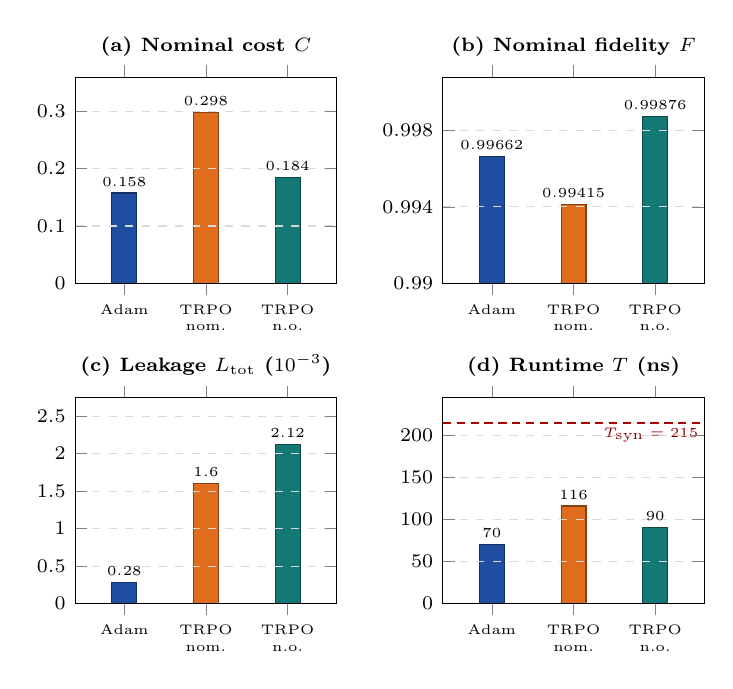
\begin{tikzpicture}
\begin{groupplot}[
  group style={group size=2 by 2, horizontal sep=1.35cm, vertical sep=1.45cm},
  metricaxis
]

% ---------------------------------------------------------------- (a) cost
\nextgroupplot[title={(a) Nominal cost $C$}, ymin=0, ymax=0.36,
               nodes near coords={\pgfmathprintnumber[fixed,precision=3]{\pgfplotspointmeta}}]
  \addplot[fill=cAdam,  draw=cAdam!60!black,  bar shift=0pt] coordinates {(Adam,0.1576)};
  \addplot[fill=cNom,   draw=cNom!60!black,   bar shift=0pt] coordinates {(Nom,0.2982)};
  \addplot[fill=cNoise, draw=cNoise!60!black, bar shift=0pt] coordinates {(NO,0.1840)};

% ------------------------------------------------------------ (b) fidelity
\nextgroupplot[title={(b) Nominal fidelity $F$}, ymin=0.990, ymax=1.0008,
               ytick={0.990,0.994,0.998},
               yticklabel style={/pgf/number format/fixed,/pgf/number format/precision=3},
               nodes near coords={\pgfmathprintnumber[fixed,precision=5]{\pgfplotspointmeta}}]
  \addplot[fill=cAdam,  draw=cAdam!60!black,  bar shift=0pt] coordinates {(Adam,0.99662)};
  \addplot[fill=cNom,   draw=cNom!60!black,   bar shift=0pt] coordinates {(Nom,0.99415)};
  \addplot[fill=cNoise, draw=cNoise!60!black, bar shift=0pt] coordinates {(NO,0.99876)};

% ------------------------------------------------------------- (c) leakage
\nextgroupplot[title={(c) Leakage $L_{\mathrm{tot}}$ ($10^{-3}$)},
               ymin=0, ymax=2.75, ytick={0,0.5,1.0,1.5,2.0,2.5},
               yticklabel style={/pgf/number format/fixed,/pgf/number format/precision=1},
               nodes near coords={\pgfmathprintnumber[fixed,precision=2]{\pgfplotspointmeta}}]
  \addplot[fill=cAdam,  draw=cAdam!60!black,  bar shift=0pt] coordinates {(Adam,0.282)};
  \addplot[fill=cNom,   draw=cNom!60!black,   bar shift=0pt] coordinates {(Nom,1.60)};
  \addplot[fill=cNoise, draw=cNoise!60!black, bar shift=0pt] coordinates {(NO,2.12)};

% ------------------------------------------------------------- (d) runtime
\nextgroupplot[title={(d) Runtime $T$ (ns)}, ymin=0, ymax=245,
               ytick={0,50,100,150,200},
               nodes near coords={\pgfmathprintnumber[fixed,precision=0]{\pgfplotspointmeta}}]
  \draw[red!65!black, dash pattern=on 3pt off 2pt, thick]
      (rel axis cs:0,{215/245}) -- (rel axis cs:1,{215/245});
  \node[font=\tiny, red!55!black, anchor=north east, inner sep=1pt]
      at (rel axis cs:0.99,{213/245}) {$T_{\mathrm{syn}}=215$};
  \addplot[fill=cAdam,  draw=cAdam!60!black,  bar shift=0pt] coordinates {(Adam,70)};
  \addplot[fill=cNom,   draw=cNom!60!black,   bar shift=0pt] coordinates {(Nom,116)};
  \addplot[fill=cNoise, draw=cNoise!60!black, bar shift=0pt] coordinates {(NO,90)};

\end{groupplot}
\end{tikzpicture}
\end{document}
